\documentclass[12pt]{article}

% ---------- Packages ----------
\usepackage[margin=1in]{geometry}   
\usepackage{graphicx}               
\usepackage{amsmath, amssymb}      
\usepackage{booktabs}               
\usepackage{hyperref}             
\usepackage{float}                  
\usepackage{caption}               
\usepackage{xcolor}                 
\usepackage{tikz}
\usetikzlibrary{positioning, arrows.meta, fit}

\usepackage[
    backend=biber,
    style=apa,
    citestyle=authoryear,
]{biblatex}
\addbibresource{refs.bib}



\hypersetup{
  colorlinks=true,
  linkcolor=blue,
  citecolor=blue,
  urlcolor=blue
}

\title{\textbf{Inferring Cuba's Hidden Economy: A Bayesian Latent Variable Model}}
\author{Christopher M. Perez}
\date{May 12, 2025}

\begin{document}
\maketitle
\tableofcontents
\newpage

\section{Introduction}
\label{sec:intro}

Measuring economic well-being in Cuba is notoriously difficult due to scarce and unreliable official statistics. The World Bank's open data portal lacks many poverty and inequality metrics for Cuba, and even basic metrics like GDP growth are contested---recent figures suggest an annual growth rate of just 1.4\% \parencite{worldbankcuba}. In the absence of trustworthy ground data, researchers increasingly turn to satellite-based proxies. Nighttime lights, for example, strongly correlate with economic output in data-sparse regions, and Cuba's contrast to  Florida in nighttime imagery highlights its economic constraints \parencite{steele2017poverty}.

In light of these data limitations, we adopt a statistical framework that infers latent economic activity using observable satellite-based proxies. This approach enables us to sidestep the need for unreliable or unavailable ground truth by utilizing spatial patterns in open geospatial data. By integrating multiple noisy indicators (nighttime lights, vegetation greeness, and road infrastructure) into a unified model, we aim to recover a smooth, yet flexibile representation of economic variation across Cuba. The goal is not to estimate GDP in absolute terms, but rather to construct a relative, spatially resolved index of economic intensity that reflects the underlying development patterns. A Bayesian framework provides both prarameter uncertainity and spatial regularization, offering us a tool for economic inference in data-scare settings. 

\section{Data Sources}

I utilize three geospatial proxies for economic activity in Cuba, all aligned on a 500 m grid. The first two sources were extracted via Google Earth Engine; the third source was directly downloaded from Geofabrik and then processed. All data correspond to the 2024 year.


\label{sec:data}
\begin{itemize}
  \item \textbf{Nighttime Lights (VIIRS):} Satellite-measured night light intensity, a well-known proxy for economic output. Brighter areas tend to indicate higher population density, infrastructure, and GDP.
  \item \textbf{NDVI (Vegetation):} The Normalized Difference Vegetation Index captures “greeness.” While high NDVI often signifies productive agriculture or healthy ecosystems, it can also be inversely correlated with poverty in some contexts.
  \item \textbf{Road Density:} Measures the density of roads, reflecting infrastructure. Well-connected regions tend to be more economically active.

\end{itemize}

The data is exported in the form of \textit{rasters}, consisting of a grid of pixels arranged in rows and columns. All rasters were reprojected and resampled to a common grid and then clipped to Cuba's extent. Across all three layers, I also masked out water pixels so that we only consider land areas. Each proxy is also standardized. This allows our model to treat each proxy on comparable footing and yields a unitless latent economic index.

\section{Bayesian Hierarchical Model}
\label{sec:model}

We define a latent variable $z_i$ for each grid cell $i$, representing the underlying economic activity (on an arbitrary scale). The observed proxies are linked to $z_i$ via a linear model:

\subsection{Observation Model}
For grid cell~$i$ and proxy~$k$:
\[
x_{i,k} \;\sim\; \mathcal{N}\!\bigl(\beta_k\,z_i,\;\sigma_k^2\bigr),
\qquad
k \in \{\text{lights},\;\text{NDVI},\;\text{roads}\},
\]

where $\beta_k$ is a weight (slope) and $\sigma_k$ is the noise standard deviation for proxy $k$. This implies that each proxy is a noisy linear indicator of the same latent $z_i$. For example, nighttime light intensity $x_{i,\text{lights}}$ is modeled as: $z_i \cdot \beta_{\text{lights}} + \text{noise}$.

\subsection{Identifiability Constraint}
To address the identifiability issue, let us fix $\beta_{\text{lights}}=1$, a unit coefficient on lights. This anchors the latent scale such that an increase of 1 in $z$ corresponds to one standard deviation increase in night lights. 

The other coefficients have weakly informative priors: $\beta_{\text{NDVI}},\,\beta_{\text{roads}} \sim \mathcal N(0,1)$. This allows NDVI and road density to be learned as either positive or negative indicators of $z$. By fixing the lights coefficient, we remove the degeneracy in scaling and ensure a unique solution for the latent field (if we instead left all $\beta$ free, the posterior would have a ridge of equal likelihood for $(z, \beta)$ rescalings).


\subsection{Spatial ICAR Prior and Neighborhood Smoothing}

In our model, we include a spatial random effect modeled with an Intrinsic Conditional Auto-Regressive (ICAR) prior. This prior introduces spatial smoothing by enforcing that neighboring areas have similar random-effect values. This is achieved using the adjacency matrix of the grid cells, which is a square matrix where each element $A_{ij}$ is 1 if cell $i$ and cell $j$ are neighbors and 0 otherwise. Under this prior, each area's effect is conditioned on the average of its neighbors' effects. In practice, we add a prior potential
\[
\;\propto\;
\exp\!\left\{-\frac{\tau}{2}\sum_{(i,j)\in\mathcal N}(z_i-z_j)^2\right\},
\]
where $\mathcal N$ is the set of neighbor pairs, and where $\tau$ is the spatial precision parameter. 

The primary advatange of using an ICAR prior is the localized smoothing it provides. The model will produce more reliable estimates for each area by pooling information with its neighbors. This is especially helpful for areas with sparse data. As a result, the posterior estimates of the spatial effects tend to be less noisy and more spatially coherent. Additionally, it also maintains local distinctness in that each area is mainly informed by its immediate neighbors, rather than enforcing a single global effect.

However, a concern with ICAR is the issue of spatial confounding, which occurs when a spatially-structured random effect competes with or masks the effects of spatially correlated covariates. In our analysis, we remain mindful of this issue so that it does not inadvertently obscure the estimated effects of our proxies.


\subsection{Weakly Informative Priors}

For the variance parameters in the model, namely ther spatial precision $\tau$ and the standard deviations $\sigma_k$, I use weakly informative priors. Specifically $\tau, \sigma_k \sim \text{HalfNormal}(1)$. This choice allows us to have some regularization: it provides some information to prevent extreme or implausible values of the variance parameters without being too strongly constraining. This type of weakly informative prior is common in hierarchical models, as it can help improve convergence and guards against overly diffuse posteriors without contributing too much bias \parencite{gelman2006prior}.


Moreover, we use a non‑centered parameterization: $z_i = \dfrac{z_i^{\mathrm{raw}}}{\sqrt{\tau}},\; z_i^{\mathrm{raw}}\sim\mathcal N(0,1)$. This lets us decouple the highly correlated magnitude of $z$ and $\tau$ and tries to avoid sampling difficulties.


\begin{figure}[H]
  \centering
  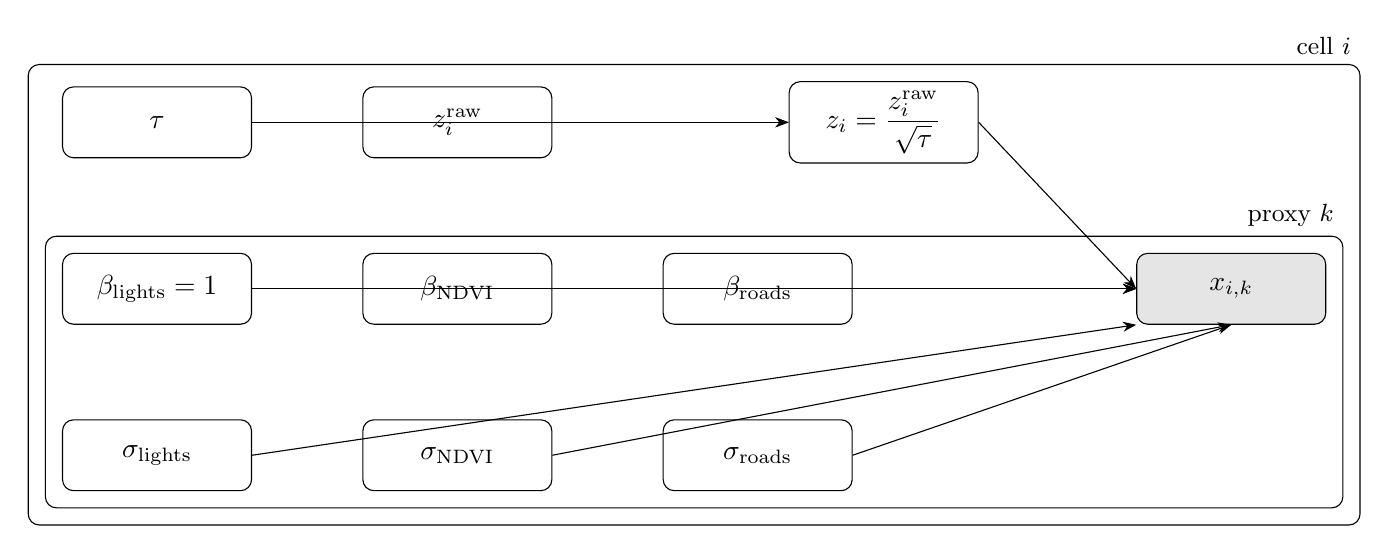
\begin{tikzpicture}[
      node distance = 12mm and 14mm,
      latent/.style  = {draw, rounded corners, minimum width=24mm, minimum height=9mm},
      param/.style   = {draw, rounded corners, minimum width=24mm, minimum height=9mm},
      obs/.style     = {draw, rounded corners, fill=gray!20, minimum width=24mm, minimum height=9mm},
      plate/.style   = {draw, rounded corners, inner sep=6pt},
      >={Stealth[]}
  ]

  % --- Latent precision and raw field ---
  \node[param]  (tau)   {$\tau$};
  \node[latent, right=of tau] (zraw) {$z^{\mathrm{raw}}_i$};
  \node[latent, right=30mm of zraw] (z)
        {$\displaystyle z_i = \frac{z^{\mathrm{raw}}_i}{\sqrt{\tau}}$};

  \draw[->] (tau) -- (z);     % tau influences z
  \draw[->] (zraw) -- (z);    % z_raw influences z

  % --- Loadings (betas) ---
  \node[param, below left=of zraw] (betaL) {$\beta_{\mathrm{lights}} = 1$};
  \node[param, right=of betaL]     (betaN) {$\beta_{\mathrm{NDVI}}$};
  \node[param, right=of betaN]     (betaR) {$\beta_{\mathrm{roads}}$};

  % --- Noise scales (sigmas) ---
  \node[param, below=of betaL] (sigL) {$\sigma_{\mathrm{lights}}$};
  \node[param, right=of sigL]  (sigN) {$\sigma_{\mathrm{NDVI}}$};
  \node[param, right=of sigN]  (sigR) {$\sigma_{\mathrm{roads}}$};

  % --- Observed variable ---
  \node[obs, right=36mm of betaR] (xik) {$x_{i,k}$};

  % --- Arrows into x_{i,k} ---
  \draw[->] (z.east)  -- (xik.west);       % z -> x
  \draw[->] (betaL.east) -- (xik.west);
  \draw[->] (betaN.east) -- (xik.west);
  \draw[->] (betaR.east) -- (xik.west);
  \draw[->] (sigL.east) -- (xik.south west);
  \draw[->] (sigN.east) -- (xik.south);
  \draw[->] (sigR.east) -- (xik.south);

  % --- Plates --------------------------------------------------
  \node[plate, fit=(betaL) (betaN) (betaR) (sigL) (sigN) (sigR) (xik)] (plateK) {};
  \node at (plateK.north east) [anchor=south east, font=\small] {proxy $k$};

  \node[plate, fit=(tau) (zraw) (z) (plateK)] (plateI) {};
  \node at (plateI.north east) [anchor=south east, font=\small] {cell $i$};

  \end{tikzpicture}
  \caption{Graphical model of the Bayesian latent‐variable hierarchy.  Precision $\tau$ rescales raw latent draws $z^{\mathrm{raw}}_i$ to give spatial latent activity $z_i$.  Observed proxies $x_{i,k}$ have Gaussian likelihood with mean $\beta_k z_i$ and noise $\sigma_k$.  A fixed loading $\beta_{\mathrm{lights}}=1$ sets the latent scale.}
  \label{fig:gm_cuba}
\end{figure}


\section{Posterior Results for Cuba (15 km Grid)}

After sampling the posterior with MCMC, we obtain the latent economic activity index $z_i$ across Cuba. Figure \ref{fig:posterior_map_round1} shows the posterior mean of $z_i$ for each 15 km grid cell across Cuba (I aggregated the 500m predictions to a coarser grid for easier visualization and computation; see next section for more). 

\begin{figure}[H]
  \centering
  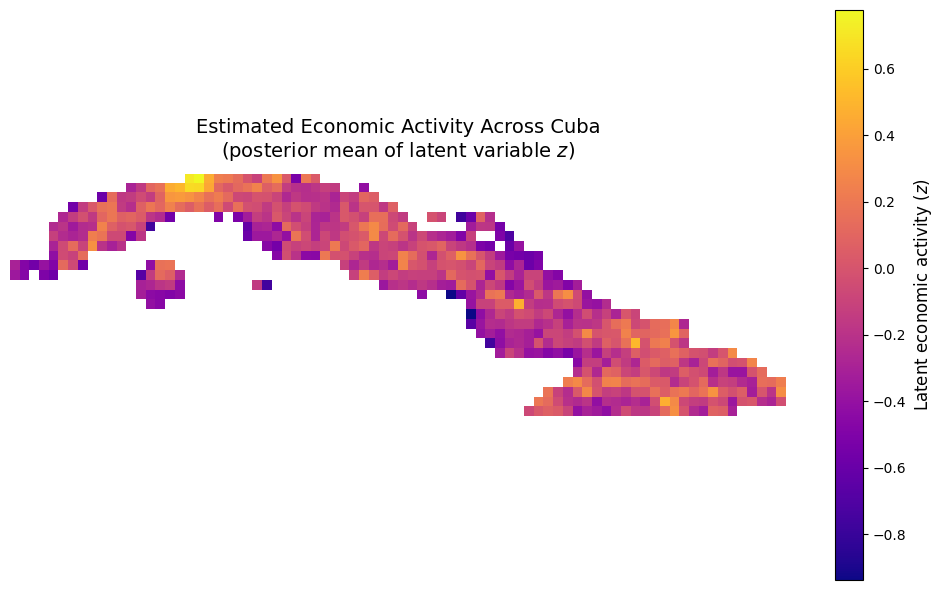
\includegraphics[width=0.6\textwidth]{/Users/chrisperez/Desktop/stat288-finalproject/images/fig1.png}
  \caption{Estimated latent economic activity index $z_i$ across Cuba.}
  \label{fig:posterior_map_round1} 
\end{figure}

Higher $z$ (yellow) denotes greater inferred economic activity, while lower $z$ (purple) denotes less. As expected, the model identifies major urban and industrial centers as hiaving the highest latent activity. For example, the capital Havana and surrounding area show up as a clear hot spot. Other major cities like Santiago de Cuba in the southeast also have relatively high activity. In contast, sparsley populated rural regions in the interior and parts of eastern Cuba have low $z$. The latent index thus reconstructs a plausible spatial pattern of economic activity consistent with qualitative knowledge of the Cuban economy.

Figure \ref{fig:posterior_map_round1_uncertainty} shows the posterior standard deviation of the $z_i$ (i.e. uncertainty of the latent index) for each location. Notably, the uncertainty is quite low overall, on the order of 0.04-0.06 in the standardized latent units. This indicates that the model is quite confident in its estimates across most of the country. 

\begin{figure}[H]
  \centering
  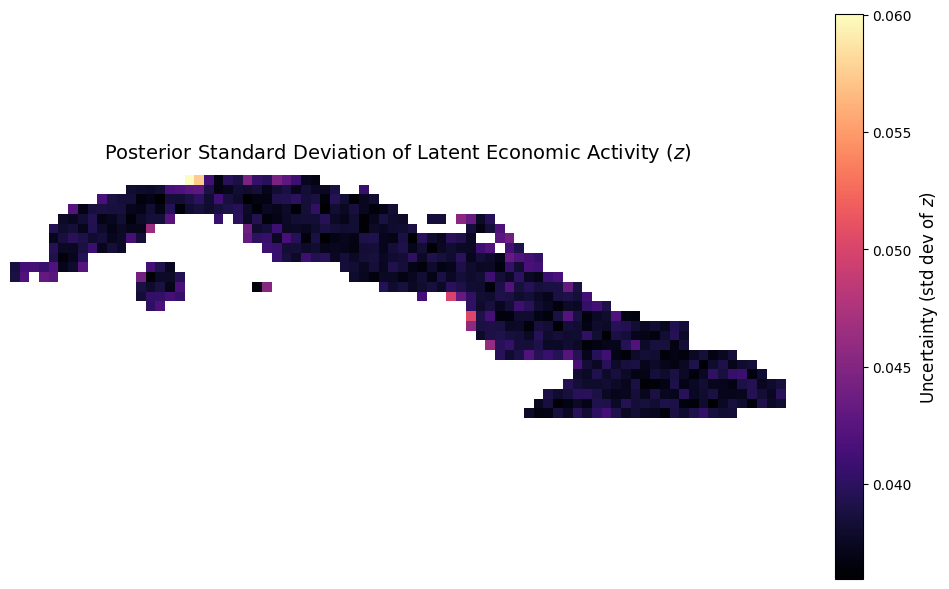
\includegraphics[width=0.6\textwidth]{/Users/chrisperez/Desktop/stat288-finalproject/images/fig2.png}
  \caption{Estimated latent economic activity index $z_i$ across Cuba.}
  \label{fig:posterior_map_round1_uncertainty} 
\end{figure}

However, we do see that there is some uncertainty in the model's estimates, particularly in the greater-Havana area. Remote rural cells, by contrast, are essentially uniformly dark.

The learned regression coefficients provide insight into each proxy's contribution (see Figure \ref{fig:marginal_posterior_plot}). We observe that $\beta_{\text{NDVI}} \approx 0.143$ and $\beta_{\text{roads}} \approx 2.289$. Nightlights have a unit coefficient, so the latent scale is directly tied to the nightlights intensity. These values suggest that, in Cuba, road density is the most strongly correlated with the latent economic factor. NVDI has a small positive coefficient, implying that geener areas are slightly associated with higher economic activity when controlling for lights and roads, but we do note that this the NVDI effect is quite weak, as the 95\% CI for this coefficient includes 0.

In terms of the noise-scale posteriors, the posterior mean for $\sigma_{\text{lights}} \approx 0.395$, $\sigma_{\text{NDVI}} \approx 1.082$, and $\sigma_{\text{roads}} \approx 0.080$. This suggests that nightlights are a fairly clean signal, while NVDI is much noiser and that greeness may contain a large amount of variation unrelated to economic activity. The road density looks almost noise-free, but it is important to note that the $\hat R$ is high (1.501), which could be explained by the extreme sparsity of the road raster - most coarse cells are exactly 0 and a few are non-zero.

\begin{figure}[H]
  \centering
  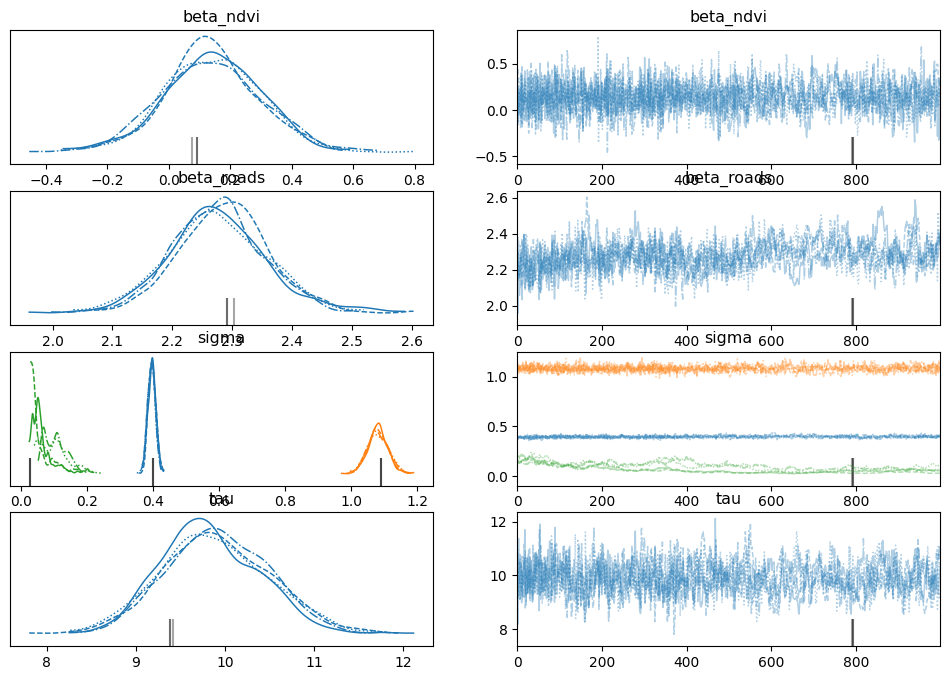
\includegraphics[width=0.8\textwidth]{/Users/chrisperez/Desktop/stat288-finalproject/images/fig_3_post_diagnostics.png}
  \caption{Marginal Posteriors (left) and MCMC Trace Plots (right) for the model parameters.}
  \label{fig:marginal_posterior_plot} 
\end{figure}





\textbf{Model Uncertainty and Limitation:} even though the statistical uncertainty is quite low, there are some caveats. The latent $z$ is an index that is only defined up to a scale and offset - it is not calibrated to an official metric like GDP per capita. Thus, while we can say one area's $z$ is higher than another's, we cannot directly interpret the difference in dollars or any absolute unit. Moreover, the model assumes the relationships (betas) are constant across space, so any spatial variation in the betas is not captured. The ICAR prior, however, tries to enforce smootheness, which can cause bleed-over over $z$ between adjacent cell. This could also cause real economic discontinuities to be smoothed out. Nonetheless, the Bayesian framework provides a principled way to quanitfy our uncertainty about the latent index $z_i$ through combining multiple data sources.



\section{Multi‑Resolution Analysis}
\label{sec:multires}

We now refit the entire Bayesian model on three alternative spatial grids obtained by averaging the original 500 m rasters into square blocks of (i) 5 km, (ii) 10 km, and (iii) 20 km.

\subsection{Variance versus Uncertainty}

Spatial varaince of the latent field increases as we move from 5 km to 20 km cells (from 0.050 to 0.105). This is expected, as coarser aggregation combines heterogeneous neighborhoods, so each super-cell becomes an average of diverse areas. Differences between super-cells therefore represent larger-scale contrasts and inflate the between-cell variance.

\subsection{Proxy Coefficients across Resolutions}
Night-lights remain the unit anchor at every resolution. We observe two interesting patterns emerge. 

First, $\beta_{\text{roads}}$ declines from 4.440 at 5 km to 3.061 at 20 km. This could be since fine grids isolate individual road segments, so coarse grids merge them together with roadless areas and thus dilute the roads-activity relationship.

Second, $\beta_{\text{NDVI}}$ flips sign. At a 5 km resolution, it is slightly negative, at -0.276. However, as we increase the grid size, the coefficient becomes positive, and at 20 km, it is 0.676. 

The resolution experiment thus strengthens the choice to keep a global variable for each proxy. For the most part, the coefficients are quite stable across resolutions even when the grid size changes. Allowing $\beta_k$ to vary by location would also introduce hundreds of extra parameters, but the data only offer three proxies per cell, which is far too little inforamtion to identify spatially varying coefficients. We have the ICAR prior help handle spatial heterogeneity, so we do not need to introduce additional parameters. Finally, this choice allows us to meaningfully compare how $\beta_{\text{roads}}$ and $\beta_{\text{NDVI}}$ vary across resolutions.

\subsection{Spatial Smoothness}
We also observe that the posterior $\tau$ drops from 17.389 to 7.023 with coarser grids, meaning that the model tolerates larger absolute differences between neighboring cells. 

\begin{figure}[H]\centering
  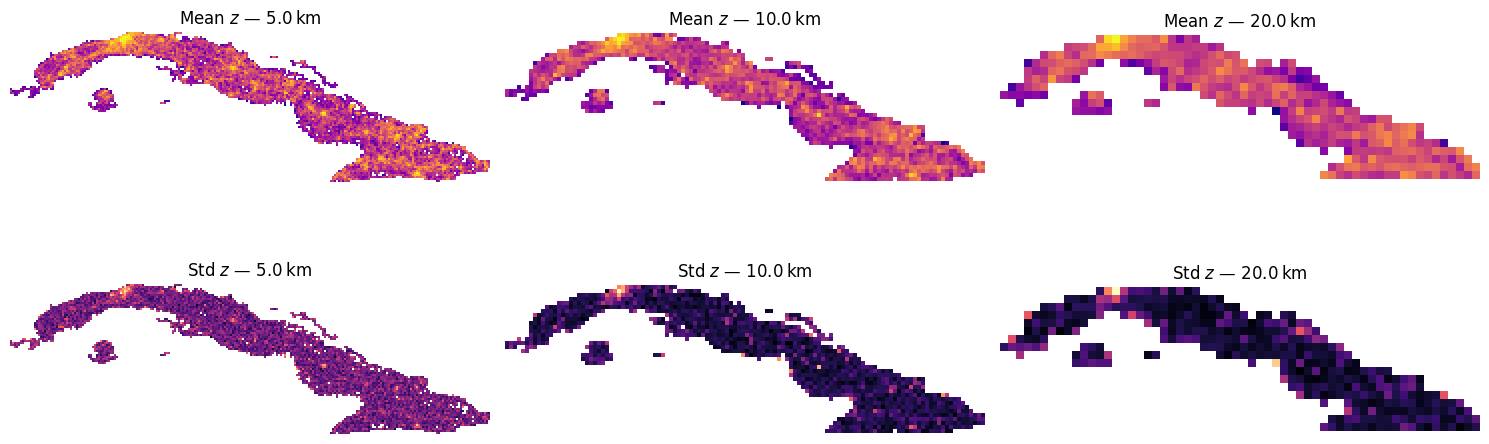
\includegraphics[width=\textwidth]{/Users/chrisperez/Desktop/stat288-finalproject/images/multires_cuba.png}
  \caption{Posterior mean (top row) and posterior standard deviation (bottom row) of latent economic activity for 5 km, 10 km, and 20 km grids.}
  \label{fig:multires_maps}
  \end{figure}
  
  \begin{figure}[H]\centering
  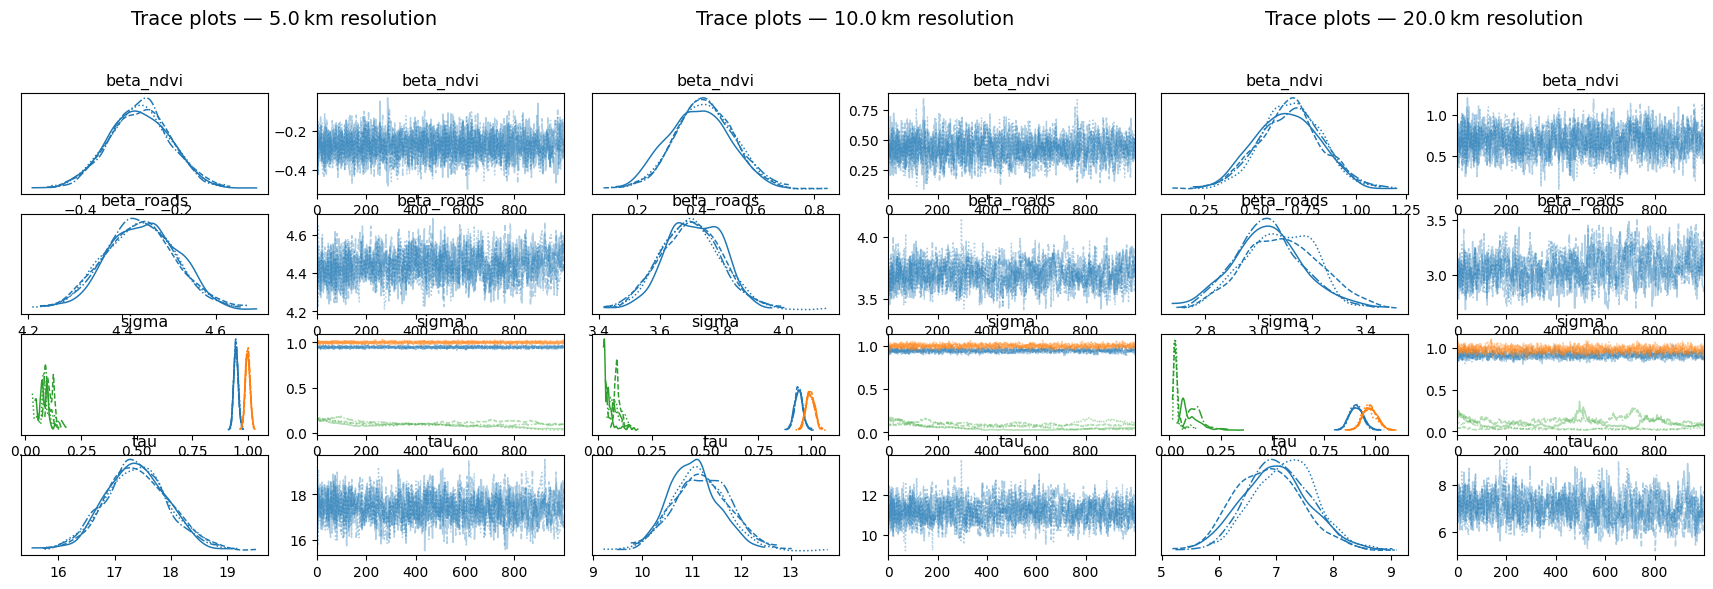
\includegraphics[width=\textwidth]{/Users/chrisperez/Desktop/stat288-finalproject/images/combined_trace_plots.png}
  \caption{Trace plots at 5 km, 10 km, and 20 km.}
  \label{fig:multires_trace}
  \end{figure}
  

\subsection{Zoom-in Comparisons: Greater Havana and Camagüey}

Figure \ref{fig:multires_zoom} displays posterior mean (top row) and posterior standard deviation (bottom row) of latent economic activity for two regions at the three resolutions previously considered: (i) Greater Havana, an urban core, and (ii) Camagüey, a largely inland province. 


\begin{figure}[H]\centering
  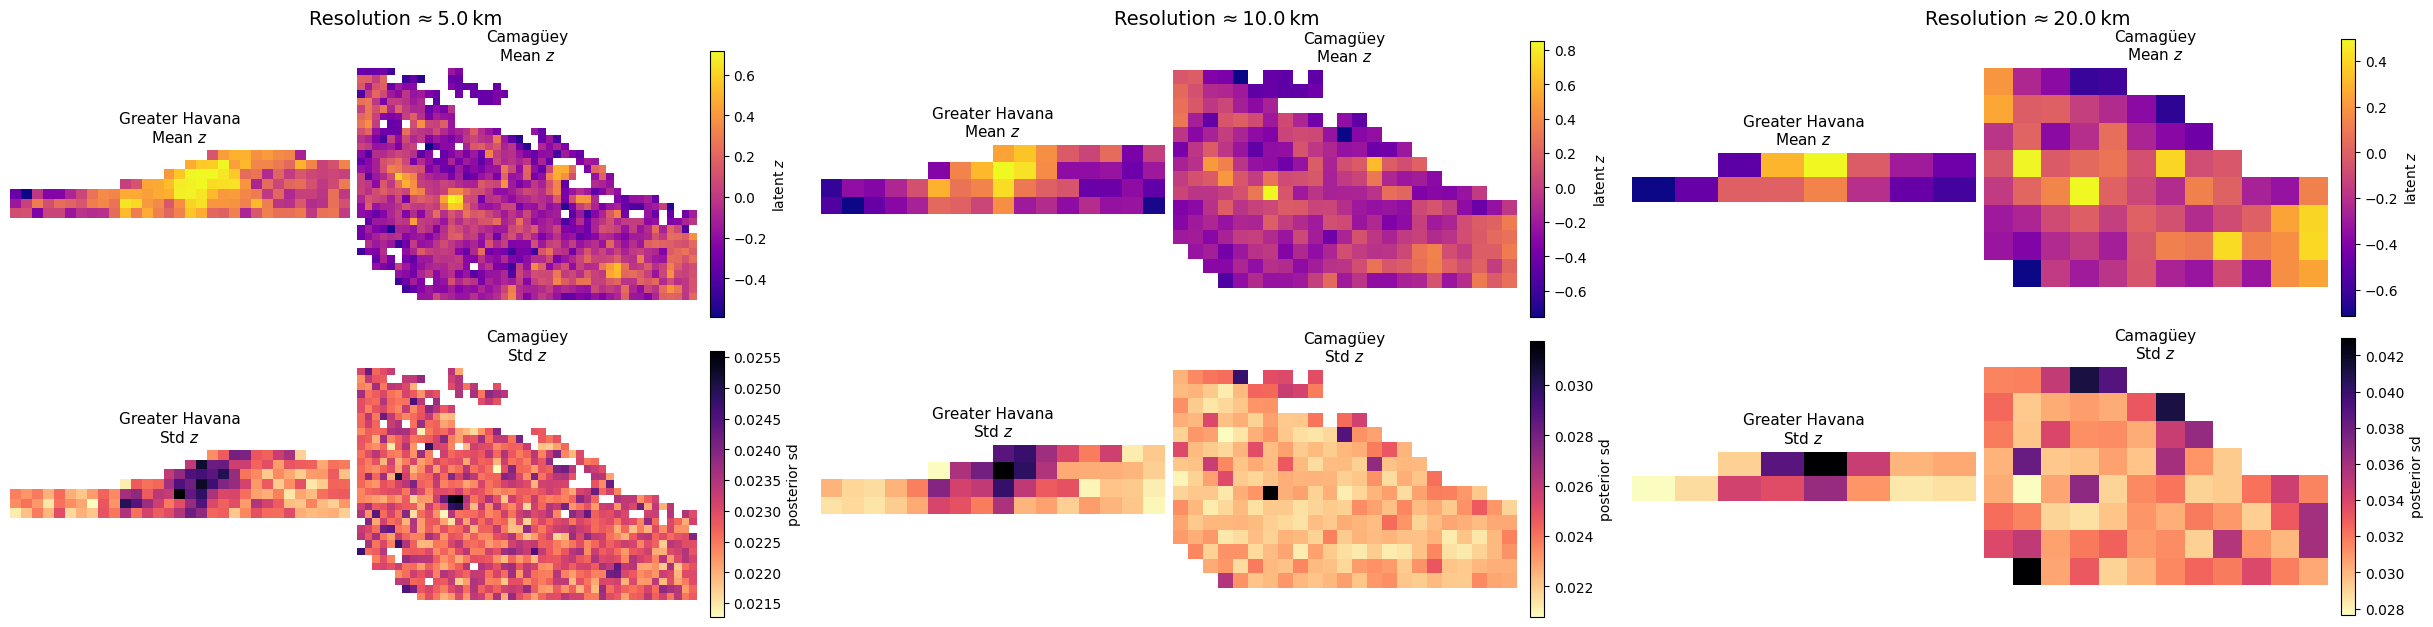
\includegraphics[width=\textwidth]{/Users/chrisperez/Desktop/stat288-finalproject/images/combined_maps.png}
  \caption{Resolution-dependent posterior mean (top) and uncertainty (bottom) for Greater Havana (left sub-panel in each column) and Camagüey (right sub-panel).}
  \label{fig:multires_zoom}
  \end{figure}

One interesting observation is that, contrary to the country-wide averages, the per-cell standard deviation actually rises with coarsening inside each zoom window. One idea is that $\tau$ decreases with block size, so the ICAR prior allows larger jumps in the latent field as we move to coarser grids. And two, each 20 km super-pixel mixes a diverse set of cells (urban plus suburbs plus rural), so the model is expressing extra uncertainty with respect to $z$.
  
  
  
  
  
  
  
  
\section{Cross‑Country Validation: Dominican Republic}
\label{sec:validation}

To assess the external validity of my latent economic activity model, I now conduct a cross-country comparison using the Dominican Republic (DR) as a benchmark. The DR was chosen for three main reasons: (1) it shares geographic, environmental, and developmental similarities with Cuba, making it a reasonable comparison case; (2) it has better coverage of socioeconomic statistics and independent validation datasets; and (3) high-resolution data on wealth is publicly available, allowing spatially granular evaluation of the model outputs.

For validation, I use Meta's \textit{Relative Wealth Index} (RWI), a dataset of wealth microestimates for 93 low- and middle-income countries (Cuba is not included!). The RWI is built from a combination of de-identified mobile phone connectivity data, satellite imagery, and machine learning techniques, and provides estimates of relative household wealth at a 2.4 km resolution across the DR \parencite{chi2022microestimates}. This data is independent of the three proxies used in my model, making the RWI an ideal source of ground-truth comparison.

To compare with my model, I first apply the same Bayesian latent variable framework to the DR using the three aligned raster proxies. After aggregating to the four different grid sizes and estimating the posterior mean latent index \( z \), I map each RWI location's latitude and longitude to its corresponding coarse cell. Each RWI data point is then assigned the model-estimated \( z \) value at its location. After filtering to points with both a valid RWI and \( z \), I calculate the Pearson correlation between the two series. The results are shown below in Figure \ref{fig:rwi_validation}.

\begin{figure}[H]
  \centering
  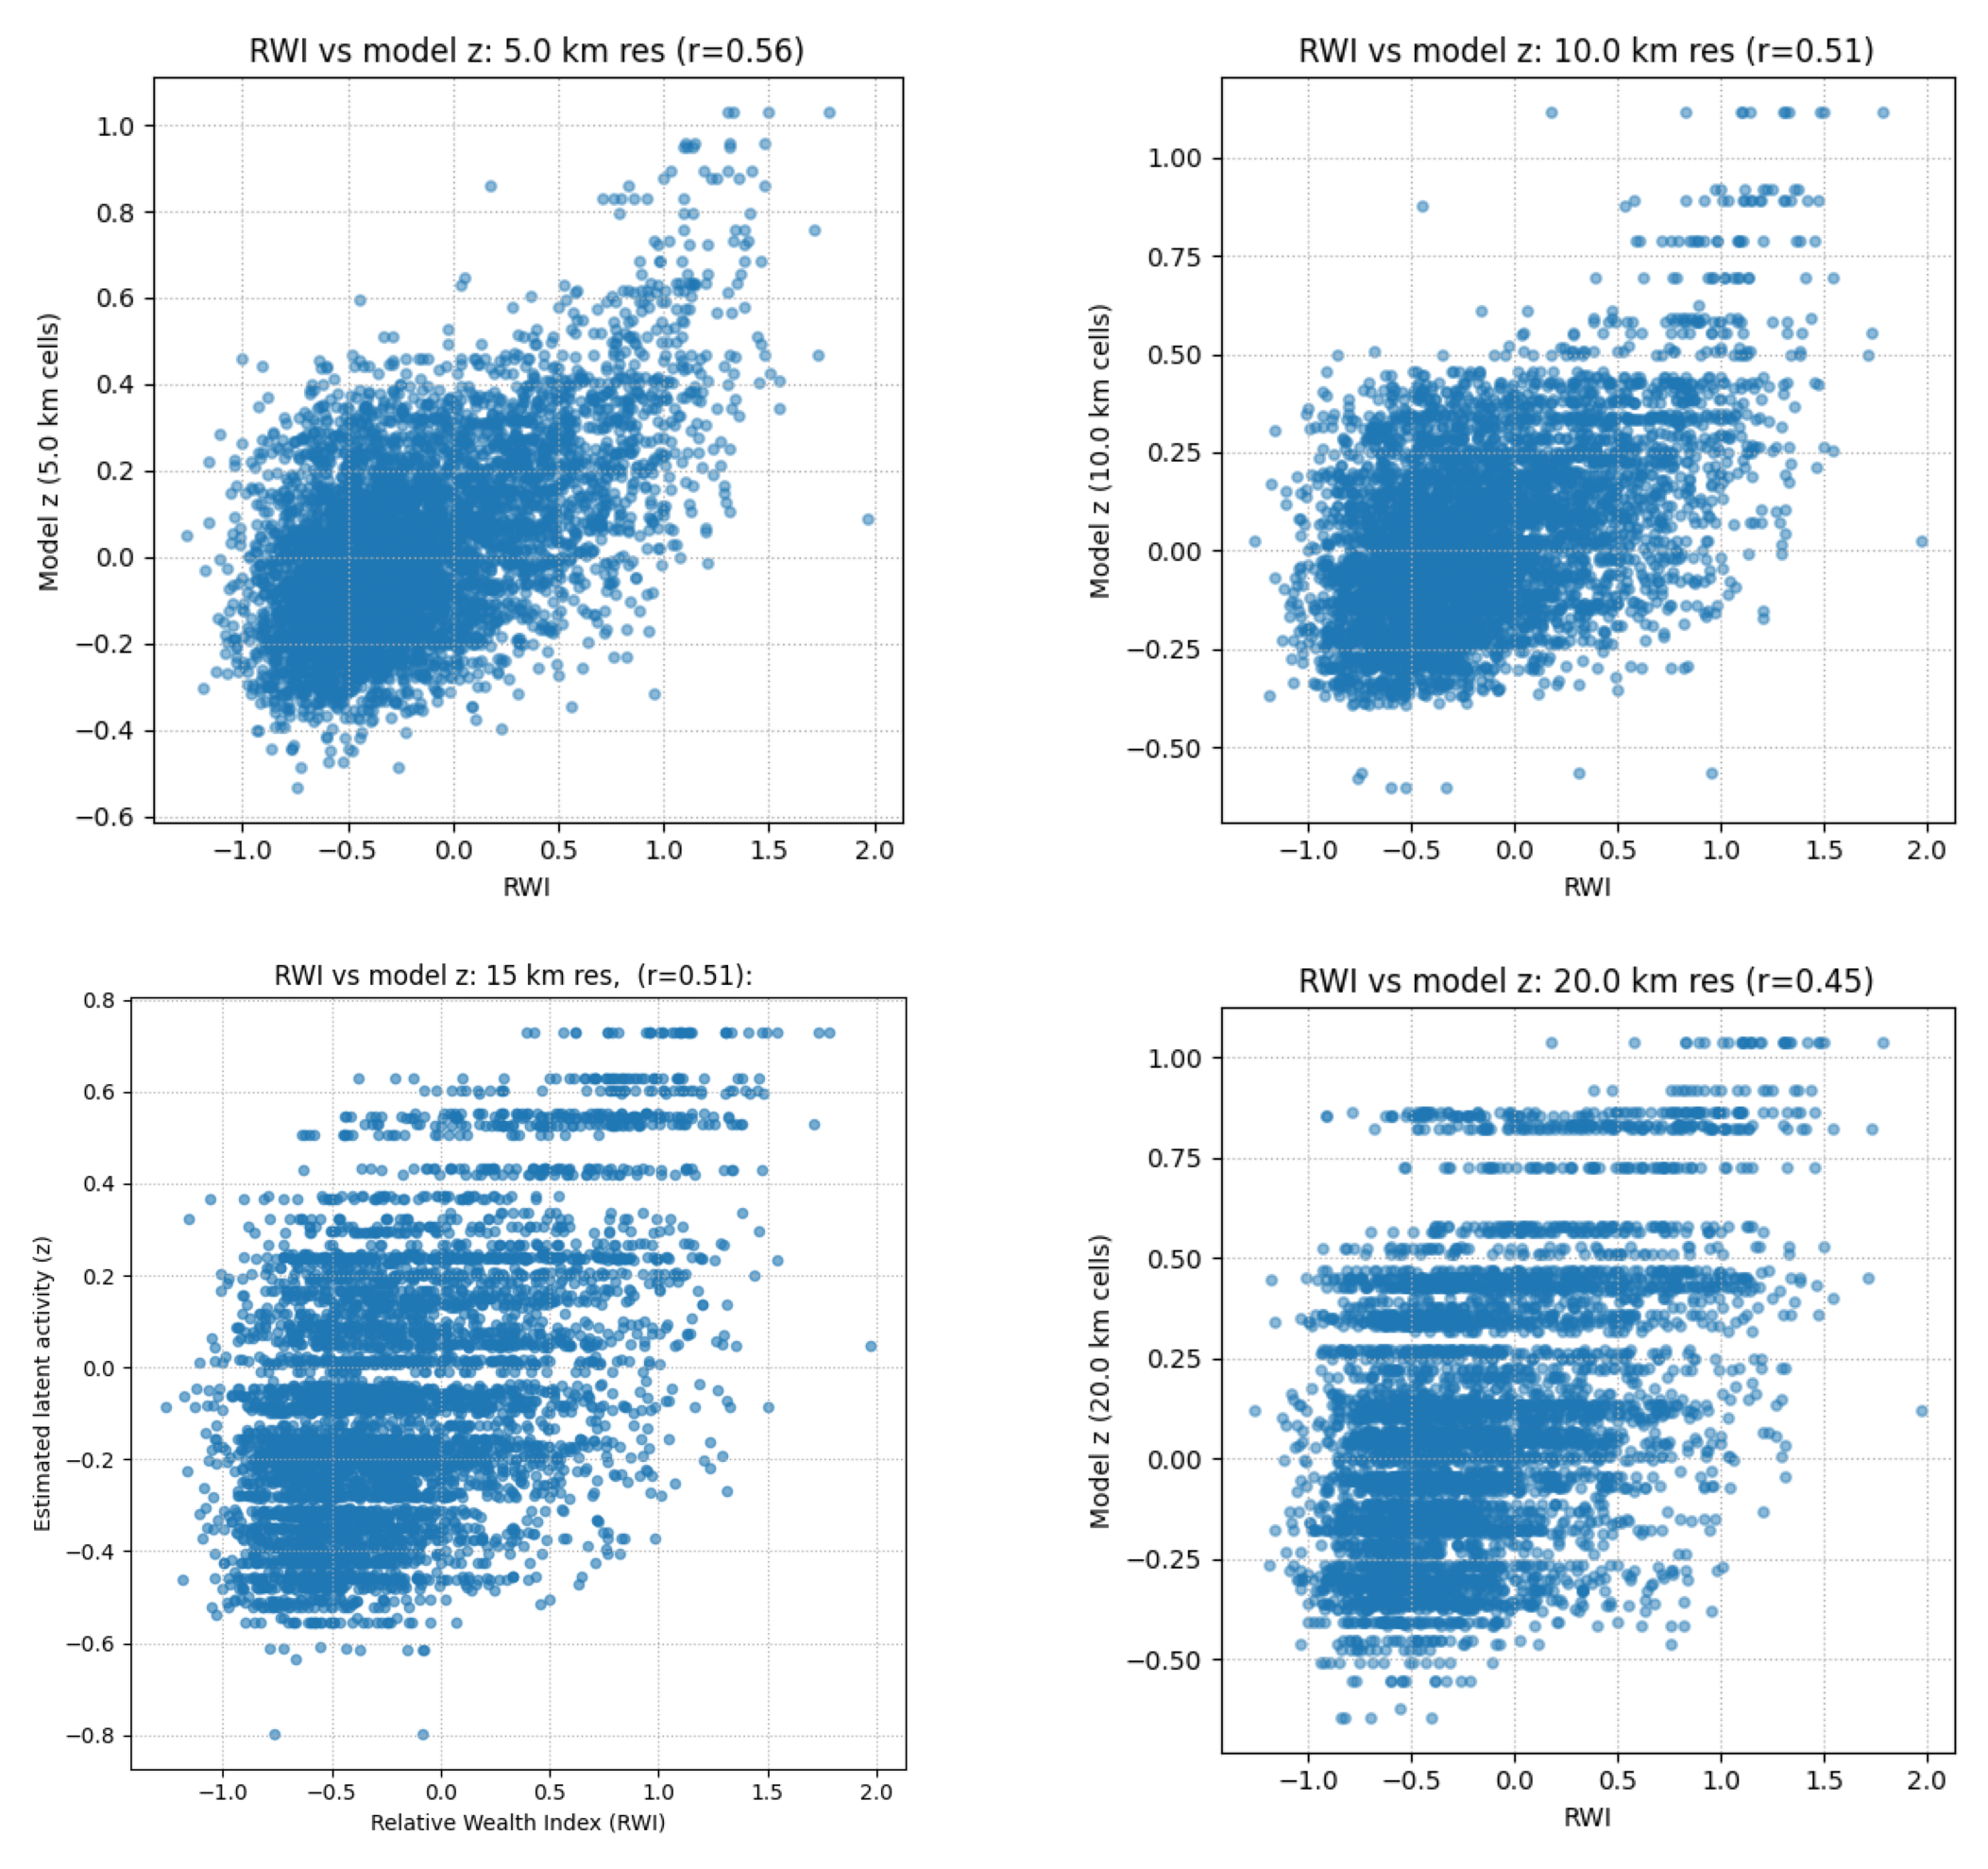
\includegraphics[width=0.7\textwidth]{/Users/chrisperez/Desktop/stat288-finalproject/images/rwi_vs_z_corr.png}
  \caption{Comparison of model-estimated latent activity ($z$) with Meta’s Relative Wealth Index (RWI) across spatial resolutions.}
  \label{fig:rwi_validation}
\end{figure}

Overall, the validation results show a consistent positive correlation between the model's estimated latent economic activity and the RWI across all spatial resolutions. At a 5 km resolution, the correlation is strongest at $r = 0.56$. But as the resolution becomes coarser, the correlation gradually weakens, from $r = 0.51$ at both 10 km and 15 km, down to $r = 0.45$ at 20 km. This trend reflects the expected trade-off: coarser grids average over heterogeneous areas and smooth out localized wealth differences. Nevertheless, the moderate correlation even at 20 km affirms that the model captures meaningful economic signals. 

Another interesting observation is the increasing hetereoskedasticity at finer spatial resolutions, particularly at 5 km and 10 km. While the strongest correlation is at 5 km, the spread of $z$ values is noticeably wider at higher RWI levels, suggesting that the model is more variable in wealthier areas. This does match what we observe with our model's posterior standard deviation in wealthier areas like Greater Havana. 





\section{Conclusion}
\label{sec:discussion}

In this project, I developed a Bayesian hierarchial model to infer a latent economic index of economic activity in Cuba from multiple proxy measurements. By combining nighttime light intensity, vegetation greener, and raod density within a single latent variable framework, I constructed a fine-grained economic activity map that is spatially coherent and plausible. The inclusion of an ICAR prior in the model enabled neighboring areas to have similar latent values, yielding smooth transitions that align with Cuba's known geographic and urban-rural patterns. 

Importantly, we externally validated the approach. When applied to the DR, the inferred latent index showed a strong correspondence with Meta's RWI, a benchmark of local wealth. This validation in a data-rich context lends credibility to our Cuba results.

Despite these promising results, several limitations of our approach need to be acknowledged. First, the estimated latent economic index is on a relative scale; it is not anchored to absolut economic units like GDP or income, which means the values indicate relative differences but not the actual size of economic output. Second, our proxy data coverage is limited: nighttime lights, vegetation, and road density each capture only certain facets of economic activity, so sectors outside their scope (for example, informal economies) may not be well represented. Additionally, the use of a spatial smoothing prior introduces the risk of spatial confounding and potential over-smoothing.

Future work could include: calibrating the latent index against ground-truth economic data where available, so that the index can be translated into absolute economic terms; incorporating additional or alternative proxies, such as mobile phone usage patterns, and detailed land use types, to broaden the evidence base for economic activity and improve coverage of hard-to-measure sectors; and finally, refining the model itself - perhaps allowing spatially varying proxy coefficients to account for regional differences. 

\noindent \textbf{Word Count:} 2559

\newpage


\printbibliography

\section*{Appendix: Code}
\label{appendix:code}

All code and data processing scripts used to generate the results in this paper are available at the following GitHub repository:

\begin{center}
\href{https://github.com/cpez04/stat288-finalproject}{\texttt{https://github.com/cpez04/stat288-finalproject.}}
\end{center}

To reproduce the results, please clone the repository and follow the instructions provided in the README.

\end{document}



